% В этом файле следует писать текст работы, разбивая его на
% разделы (section), подразделы (subsection) и, если нужно,
% главы (chapter).

% Предварительно следует указать необходимую информацию
% в файле SETUP.tex

%% В этот файл не предполагается вносить изменения

% В этом файле следует указать информацию о себе
% и выполняемой работе.

\documentclass [fontsize=14pt, paper=a4, pagesize, DIV=calc]%
{scrreprt}
% ВНИМАНИЕ! Для использования глав поменять
% scrartcl на scrreprt

% Здесь ничего не менять
\usepackage [T2A] {fontenc}   % Кириллица в PDF файле
\usepackage [utf8] {inputenc} % Кодировка текста: utf-8
\usepackage [russian] {babel} % Переносы, лигатуры

%%%%%%%%%%%%%%%%%%%%%%%%%%%%%%%%%%%%%%%%%%%%%%%%%%%%%%%%%%%%%%%%%%%%%%%%
% Создание макроса управления элементами, специфичными
% для вида работы (курс., бак., маг.)
% Здесь ничего не менять:
\usepackage{ifthen}
\newcounter{worktype}
\newcommand{\typeOfWork}[1]
{
	\setcounter{worktype}{#1}
}

% ВНИМАНИЕ!
% Укажите тип работы: 0 - курсовая, 1 - бак., 2 - маг.,
% 3 - бакалаврская с главами.
\typeOfWork{2}
% Считается, что курсовая и бак. бьются на разделы (section) и
% подразделы (subsection), а маг. — на главы (chapter), разделы и
%  подразделы. Если хочется,
% чтобы бак. была с главами (например, если она большая),
% надо выбрать опцию 3.

% Если при выборе 2 или 3 вы забудете поменять класс
% документа на scrreprt (см. выше, в самом начале),
% то получите ошибку:
% ./aux/appearance.tex:52: Package scrbase Error: unknown option ` chapterprefix=

%%%%%%%%%%%%%%%%%%%%%%%%%%%%%%%%%%%%%%%%%%%%%%%%%%%%%%%%%%%%%%%%%%%%%%%%
% Информация об авторе и работе для титульной страницы

\usepackage {titling}

% Имя автора в именительном падеже (для маг.)
\newcommand {\me}{%
В.\,В.~Быцюк%
}

% Имя автора в родительном падеже (для курсовой и бак.)
\newcommand {\byme}{%
В.\,В.~Быцюка%
}

% Любимый научный руководитель
\newcommand{\supervisor}%
{старший преподаватель \\ В. Н. Брагилевский}

% Рецензент
\newcommand{\reviewer}
{кандидат физико-математических наук, доцент \\ С. А. Гуда}

% идентифицируем пол (только для курсовой и бак.)
\newcommand{\bystudent}{
Студента %Студентки % Для курсовой: с большой буквы
}

% Год публикации
\date{2018}

% Название работы
\title{Размещение реплик в распределенной системе\\на базе Erlang-процессов}

% Кафедра
%
\newboolean{needchair}
\setboolean{needchair}{true} % на ФИИТ не пишется (false), на ПМИ есть (true)

\newcommand {\thechair} {%
Кафедра информатики и вычислительного эксперимента%
}

\newcommand {\direction} {%
Направление подготовки\\
Прикладная математика и информатика%
}% Прикладная математика и информатика

%%%%%%%%%%%%%%%%%%%%%%%%%%%%%%%%%%%%%%%%%%%%%%%%%%%%%%%%%%%%%%%%%%%%%%%%
% Другие настраиваемые элементы текста

% Листинги с исходным кодом программ: укажите язык программирования
\usepackage{listings}
\lstset{
    language=erlang,%  Язык указать здесь
    basicstyle=\small\ttfamily,
    breaklines=true,%
    showstringspaces=false%
    inputencoding=utf8x%
}
% полный список языков, поддерживаемых данным пакетом, есть,
% например, здесь (стр. 13):
% ftp://ftp.tex.ac.uk/tex-archive/macros/latex/contrib/listings/listings.pdf

% Нумерация списков: можно при необходимести
% изменять вид нумерации (например, добавлять правую скобку).
% По умолчанию буду списки вида:
% 1.
% 2.
% Изменять вид нумерации можно в начале нумерации:
% \begin{enumerate}[1)] (В квадратных скобках указан желаемый вид)
\usepackage[shortlabels]{enumitem}
                    \setlist[enumerate, 1]{1.}

% Гиперссылки: настройте внешний вид ссылок
\usepackage%
[pdftex,unicode,pdfborder={0 0 0},draft=false,%backref=page,
    hidelinks, % убрать, если хочется видеть ссылки: это
               % удобно в PDF файле, но не должно появиться на печати
    bookmarks=true,bookmarksnumbered=false,bookmarksopen=false]%
{hyperref}


\usepackage {amsmath}      % Больше математики
\usepackage {amssymb}
\usepackage {textcase}     % Преобразование к верхнему регистру
\usepackage {indentfirst}  % Красная строка первого абзаца в разделе

\usepackage {fancyvrb}     % Листинги: определяем своё окружение Verb
\DefineVerbatimEnvironment% с уменьшенным шрифтом
	{Verb}{Verbatim}
	{fontsize=\small}

% Вставка рисунков
\usepackage {graphicx}

% Общее оформление
% ----------------------------------------------------------------
% Настройка внешнего вида

%%% Шрифты

% если закомментировать всё — консервативная гарнитура Computer Modern
\usepackage{paratype} % профессиональные свободные шрифты
%\usepackage {droid}  % неплохие свободные шрифты от Google
%\usepackage{mathptmx}
%\usepackage {mmasym}
%\usepackage {psfonts}
%\usepackage{lmodern}
%var1: lh additions for bold concrete fonts
%\usepackage{lh-t2axccr}
%var2: the package below could be covered with fd-files
%\usepackage{lh-t2accr}
%\usepackage {pscyr}

% Геометрия текста

\usepackage{setspace}       % Межстрочный интервал
\onehalfspacing

\newlength\MyIndent
\setlength\MyIndent{1.25cm}
\setlength{\parindent}{\MyIndent} % Абзацный отступ
\frenchspacing            % Отключение лишних отступов после точек
\KOMAoptions{%
    DIV=calc,         % Пересчёт геометрии
    numbers=endperiod % точки после номеров разделов
}

                            % Консервативный вариант:
%\usepackage                % ручное задание геометрии
%[%                         % (не рекомендуется в проф. типографии)
%  margin = 2.5cm,
  %includefoot,
  %footskip = 1cm
%] %
%  {geometry}

%%% Заголовки

\ifthenelse{\equal{\theworktype}{2}}{%
\KOMAoptions{%
    numbers=endperiod,% точки после номеров разделов
    headings=normal,   % размеры заголовков поменьше стандартных
    chapterprefix=true,% Печатать слово Глава в магистерской
    appendixprefix=true% Печатать слово Приложение
}
}

% шрифт для оформления глав и названия содержания
\newcommand{\SuperFont}{\Large\sffamily\bfseries}

% Заголовок главы
\ifthenelse{\value{worktype} > 1}{%
\renewcommand{\SuperFont}{\Large\normalfont\sffamily}
\newcommand{\CentSuperFont}{\centering\SuperFont}
\usepackage{fncychap}
\ChNameVar{\SuperFont}
\ChNumVar{\CentSuperFont}
\ChTitleVar{\CentSuperFont}
\ChNameUpperCase
\ChTitleUpperCase
}

% Заголовок (под)раздела с абзацного отступа
\addtokomafont{sectioning}{\hspace{\MyIndent}}

\renewcommand*{\captionformat}{~---~}
\renewcommand*{\figureformat}{Рисунок~\thefigure}

% Плавающие листинги
\usepackage{float}
\floatstyle{ruled}
\floatname{ListingEnv}{Листинг}
\newfloat{ListingEnv}{htbp}{lol}[section]

% точка после номера листинга
\makeatletter
\renewcommand\floatc@ruled[2]{{\@fs@cfont #1.} #2\par}
\makeatother


%%% Оглавление
\usepackage{tocloft}

% шрифт и положение заголовка
\ifthenelse{\value{worktype} > 1}{%
\renewcommand{\cfttoctitlefont}{\hfil\SuperFont\MakeUppercase}
}{
\renewcommand{\cfttoctitlefont}{\hfil\SuperFont}
}

% слово Глава
\usepackage{calc}
\ifthenelse{\value{worktype} > 1}{%
\renewcommand{\cftchappresnum}{Глава }
\addtolength{\cftchapnumwidth}{\widthof{Глава }}
}

% Очищаем оформление названий старших элементов в оглавлении
\ifthenelse{\value{worktype} > 1}{%
\renewcommand{\cftchapfont}{}
\renewcommand{\cftchappagefont}{}
}{
\renewcommand{\cftsecfont}{}
\renewcommand{\cftsecpagefont}{}
}

% Точки после верхних элементов оглавления
\renewcommand{\cftsecdotsep}{\cftdotsep}
%\newcommand{\cftchapdotsep}{\cftdotsep}

\ifthenelse{\value{worktype} > 1}{%
    \renewcommand{\cftchapaftersnum}{.}
}{}
\renewcommand{\cftsecaftersnum}{.}
\renewcommand{\cftsubsecaftersnum}{.}
\renewcommand{\cftsubsubsecaftersnum}{.}

%%% Списки (enumitem)

\usepackage {enumitem}      % Списки с настройкой отступов
\setlist %
{ %
  leftmargin = \parindent, itemsep=.5ex, topsep=.4ex
} %

% По ГОСТу нумерация должны быть буквами: а, б...
%\makeatletter
%    \AddEnumerateCounter{\asbuk}{\@asbuk}{м)}
%\makeatother
%\renewcommand{\labelenumi}{\asbuk{enumi})}
%\renewcommand{\labelenumii}{\arabic{enumii})}

%%% Таблицы: выбрать более подходящие

\usepackage{booktabs} % считаются наиболее профессионально выполненными
%\usepackage{ltablex}
%\newcolumntype {L} {>{---}l}

%%% Библиография

\usepackage{csquotes}        % Оформление списка литературы
\usepackage[
  backend=biber,
  hyperref=auto,
  sorting=none, % сортировка в порядке встречаемости ссылок
  language=auto,
  citestyle=gost-numeric,
  bibstyle=gost-numeric
]{biblatex}
\addbibresource{biblio.bib} % Файл с лит.источниками

% Настройка величины отступа в списке
\ifthenelse{\value{worktype} < 2}{%
\defbibenvironment{bibliography}
  {\list
     {\printtext[labelnumberwidth]{%
    \printfield{prefixnumber}%
    \printfield{labelnumber}}}
     {\setlength{\labelwidth}{\labelnumberwidth}%
      \setlength{\leftmargin}{\labelwidth}%
      \setlength{\labelsep}{\dimexpr\MyIndent-\labelwidth\relax}% <----- default is \biblabelsep
      \addtolength{\leftmargin}{\labelsep}%
      \setlength{\itemsep}{\bibitemsep}%
      \setlength{\parsep}{\bibparsep}}%
      \renewcommand*{\makelabel}[1]{\hss##1}}
  {\endlist}
  {\item}
}{}

% ----------------------------------------------------------------
% Настройка переносов и разрывов страниц

\binoppenalty = 10000      % Запрет переносов строк в формулах
\relpenalty = 10000        %

\sloppy                    % Не выходить за границы бокса
%\tolerance = 400          % или более точно
\clubpenalty = 10000       % Запрет разрывов страниц после первой
\widowpenalty = 10000      % и перед предпоследней строкой абзаца

% ----------------------------


% Стили для окружений типа Определение, Теорема...
% Оформление теорем (ntheorem)

\usepackage [thmmarks, amsmath] {ntheorem}
\theorempreskipamount 0.6cm

\theoremstyle {plain} %
\theoremheaderfont {\normalfont \bfseries} %
\theorembodyfont {\slshape} %
\theoremsymbol {\ensuremath {_\Box}} %
\theoremseparator {:} %
\newtheorem {mystatement} {Утверждение} [section] %
\newtheorem {mylemma} {Лемма} [section] %
\newtheorem {mycorollary} {Следствие} [section] %

\theoremstyle {nonumberplain} %
\theoremseparator {.} %
\theoremsymbol {\ensuremath {_\diamondsuit}} %
\newtheorem {mydefinition} {Определение} %

\theoremstyle {plain} %
\theoremheaderfont {\normalfont \bfseries} 
\theorembodyfont {\normalfont} 
%\theoremsymbol {\ensuremath {_\Box}} %
\theoremseparator {.} %
\newtheorem {mytask} {Задача} [section]%
\renewcommand{\themytask}{\arabic{mytask}}

\theoremheaderfont {\scshape} %
\theorembodyfont {\upshape} %
\theoremstyle {nonumberplain} %
\theoremseparator {} %
\theoremsymbol {\rule {1ex} {1ex}} %
\newtheorem {myproof} {Доказательство} %

\theorembodyfont {\upshape} %
%\theoremindent 0.5cm
\theoremstyle {nonumberbreak} \theoremseparator {\\} %
\theoremsymbol {\ensuremath {\ast}} %
\newtheorem {myexample} {Пример} %
\newtheorem {myexamples} {Примеры} %

\theoremheaderfont {\itshape} %
\theorembodyfont {\upshape} %
\theoremstyle {nonumberplain} %
\theoremseparator {:} %
\theoremsymbol {\ensuremath {_\triangle}} %
\newtheorem {myremark} {Замечание} %
\theoremstyle {nonumberbreak} %
\newtheorem {myremarks} {Замечания} %


% Титульный лист
% Макросы настройки титульной страницы
% В этот файл не предполагается вносить изменения

%\usepackage {showframe}

% Вертикальные отступы на титульной странице
\newcommand{\vgap}{\vspace{16pt}}

% Помещение города и даты в нижний колонтитул
\usepackage{scrlayer}
\DeclareNewLayer[
  foot,
  foreground,
  contents={%
    \raisebox{\dp\strutbox}[\layerheight][0pt]{%
      \parbox[b]{\layerwidth}{\centering Ростов-на-Дону\\ \thedate%
       \\\mbox{}
       }}%
  }
]{titlepage.foot.fg}
\DeclareNewPageStyleByLayers{titlepage}{titlepage.foot.fg}


\AtBeginDocument %
{ %
  %
  \begin{titlepage}
  %
    \thispagestyle{titlepage}

    {\centering
    %
    \MakeTextUppercase {МИНИСТЕРСТВО ОБРАЗОВАНИЯ И НАУКИ РФ}

    \vgap

    Федеральное государственное автономное образовательное\\
    учреждение высшего образования\\
    \MakeTextUppercase {Южный федеральный университет}

    \vgap

	Институт математики, механики и компьютерных наук
    имени~И.\,И.\,Воровича

    \vgap

    \direction

    \ifthenelse{\boolean{needchair}}{
    \vgap

    \thechair}{}

    \vspace* {\fill}

    \ifthenelse{\value{worktype} = 2}{%
    \me

    \vgap}{}

    {\usefont{T2A}{PTSansCaption-TLF}{m}{n}
    \MakeTextUppercase{\thetitle}}

    \ifthenelse{\value{worktype} = 2}{%
     \vgap

    Магистерская диссертация}{}
    \ifthenelse{\value{worktype} = 0}{
     \vgap

    Курсовая работа
    }{}%
    \ifthenelse{\value{worktype} = 1 \OR \value{worktype} = 3}{
     \vgap

    Выпускная квалификационная работа\\
    на степень бакалавра
    }{}%

    \vspace {\fill}

    \begin{flushright}
    \ifthenelse{\value{worktype} = 0 \OR 
                \value{worktype} = 1 \OR
                \value{worktype} = 3}{
      \bystudent \ifthenelse{\value{worktype} = 0}{3}{4}\ курса\\
      \byme
    }{}

    \vgap

    Научный руководитель:\\
    \supervisor\\
    \ifthenelse{\value{worktype} = 2}{%
    Рецензент:\\
    ученая степень, ученое звание, должность
    И. О. Фамилия
    }{}
	\end{flushright}
    \ifthenelse{\value{worktype} = 0}{
    \vspace{\fill}
            \begin{flushleft}
              \begin{tabular}{cc}
                \underline{\hspace{4cm}}&\underline{\hspace{5cm}}\\
                {\small оценка (рейтинг)} & {\small  подпись руководителя}\\
              \end{tabular}
            \end{flushleft}
    }{}
  	\vspace {\fill}
  %Ростов-на-Дону

    %\thedate

  }\end{titlepage}
  %
  %
  %\tableofcontents
  %
  \clearpage
} %



% Команды для использования в тексте работы


% макросы для начала введения и заключения
\newcommand{\Intro}{\addsec{Введение}}
\ifthenelse{\value{worktype} > 1}{%
    \renewcommand{\Intro}{\addchap{Введение}}%
}

\newcommand{\Task}{\addsec{Постановка задачи}}
\ifthenelse{\value{worktype} > 1}{%
    \renewcommand{\Task}{\addchap{Постановка задачи}}%
}

\newcommand{\Conc}{\addsec{Заключение}}
\ifthenelse{\value{worktype} > 1}{%
    \renewcommand{\Conc}{\addchap{Заключение}}%
}

% Правильные значки для нестрогих неравенств и пустого множества
\renewcommand {\le} {\leqslant}
\renewcommand {\ge} {\geqslant}
\renewcommand {\emptyset} {\varnothing}

% N ажурное: натуральные числа
\newcommand {\N} {\ensuremath{\mathbb N}}

% значок С++ — используйте команду \cpp
\newcommand{\cpp}{%
C\nolinebreak\hspace{-.05em}%
\raisebox{.2ex}{+}\nolinebreak\hspace{-.10em}%
\raisebox{.2ex}{+}%
}

% Неразрывный дефис, который допускает перенос внутри слов,
% типа жёлто-синий: нужно писать жёлто"/синий.
\makeatletter
    \defineshorthand[russian]{"/}{\mbox{-}\bbl@allowhyphens}
\makeatother


\endinput

% Конец файла


\begin{document}

\Task
	\begin{enumerate}
		\item Реализовать распределенное клиент-серверное приложение 
		для хранения данных на языке программирования Erlang.
		
		\item Реализовать алгоритм размещения реплик объектов в 
		распределенной сети.
		
		\item Провести замеры времени работы алгоритма и сравнить 
		полученные результаты с результатами из статьи 
	\end{enumerate}
\newpage

\tableofcontents
\newpage

\Intro
	В данной работе реализована распределенная система на базе Erlang процессов. Она включает в себя серверные приложения хранящие пары ключ-значение и клиентские приложения,
	управляющие данными на серверах. Так же у серверов есть возможность привязываться друг к другу и отвязываться друг от друга получая HTTP запросы во время работы системы без ущерба для
	хранимых данных. Помимо этого реализован алгоритм по размещению реплик объектов на серверах системы для ускорения получения доступа к наиболее популярным для каждого сервера
	объектам системы.
	
	На полученой системе проведены сравнения времени работы алгоритма размещения реплик при различных конфигурациях системы и различном количестве объектов, а также анализ полученных 
	временных результатов.
	
	Целью работы является реализация распределенной системы и алгоритма размещения реплик, а также анализ времени его работы.
\newpage

\chapter{Обзор используемых технологий и алгоритмов}
	\section{Язык программирования Erlang и его окружение}
		Erlang --- функциональный язык программирования, созданный для разработки	распределенных динамических систем~\cite{erl}.
		Основные его преимущества: быстрая и эффективная разработка, устойчивость системы к аппаратным сбоям и 
		возможность обновления всей системы без остановки программ.

		\subsection{Переменные и атомы} 
			Переменные в Erlang начинаются с заглавной буквы. Им можно присваивать значения только один раз. 
			Переменная, которой значение уже присвоено, называется связанной. В противном случае она называется свободной. 
			Попытка присвоить связанной переменной новое значение приведет к сообщению об ошибке.
			\begin{lstlisting}
X = 42.
			\end{lstlisting}

			Атомы используются для представления нечисловых констант. Значением атома является сам атом.
			\begin{lstlisting}
monday.
			\end{lstlisting}  

		\subsection{Кортежи}
			Кортеж --- единая группа из фиксированного числа объектов. Группа является анонимной, как и каждое отдельное 
			поле кортежа. Часто первым элементом кортежа используют атом, который описывает этот кортеж.
			\begin{lstlisting}
{1, september, 2012}.
{point, 6, 7}.
			\end{lstlisting}
			
			Возможно присваивать переменным значения отдельных элементов кортежа. Символ \_ называется анонимной переменной. 
			Такой переменной не привязывается соответствующее значение.
			\begin{lstlisting}
{Name, _} = {joe, armstrong}.
			\end{lstlisting} 

		\subsection{Списки} 
			Списки используются для хранения различных данных. Головой списка называется его первый элемент. Если удалить 
			голову из списка, то останется хвост исходного списка.
			\begin{lstlisting}
[{joe, armstrong}, {1, september, 2012}, 42].
			\end{lstlisting}

		\subsection{Функции}
			Рассмотрим описание функций в Erlang на примере нахождения площади прямоугольника и круга.
			\begin{lstlisting}
area({rectangle, Width, Height}) -> Width * Height;
area({circle, Radius}) -> 3.14159 * Radius * Radius.
			\end{lstlisting}
			Функция area содержит 2 варианта сопоставления аргументов --- клаузы. Первый вариант необходим для нахождения 
			площади прямоугольника, а второй --- круга. 	
			
		\subsection{Процессы}
			Для парралельного выполнени некоторых операций в Erlang используют процессы.
			\begin{lstlisting}
Pid = spawn(Fun).
			\end{lstlisting}
			Функция spawn принимает функцию которую надо выполнить и запускает отдельный процесс. В Pid записывается идентификатор
			этого процесса, для того, чтобы в дальнейшем ему можно было обращаться.
			
			Общение между процессами происходит посредством обмена сооьщениями. Например
			\begin{lstlisting}
Pid ! Message.
			\end{lstlisting}
			отправляет сообщение Message процессу с идентификатором Pid.

			Процессы принимают сообщения с помощью конструкции recieve ... end. 
			\begin{lstlisting}
receive
	Pattern1 -> Expressions1;
	Pattern2 -> Expressions2;
	true -> Expression3
end
			\end{lstlisting}
			Каждое пришедшее сообщение сравнивается с Pattern1 и Pattern2 и в случае совпадения возвращается описанное в данной 
			ветке выражение, а если совпадения не произошло --- выбирается выражение из ветки true. 
	

	\section{Красно-черные деревья}
		Красно-черное дерево --- двоичное дерево поиска, узлы которого 
		разделены на красные (red) и черные (black). Для таких деревьев
		должны выполняться красно-черные свойства (RB properties), 
		гарантирующие, что глубины любых двух листьев отличаются не более
		чем в 2 раза~\cite{kormen}.

		Узлы красно-черного дерева обычно содержат следующие поля:
		\begin{enumerate}
			\item Значение
			\item Цвет
			\item Родитель
			\item Левый ребенок
			\item Правый ребенок
		\end{enumerate}	

		Важно отметить, что если ребенок или родитель отсутствует, то
		соответствующее поле содержит черный лист.
		
		Рассмотрим упомянутые выше красно-черные свойства:
		\begin{enumerate}
			\item Каждый узел дерева --- либо красный, либо черный.
			\item Корень дерева --- черный.
			\item Каждый лист --- черный.
			\item Если узел красный, то оба его ребенка черные.
			\item Все простые пути, идущие от корня к листьям, содержат 
				  одинаковое количество черных узлов.
		\end{enumerate}
		
		Для удобства работы все листья заменяются одним черным листом.
		Это обычный узел дерева со значением nil, черным цветом и произвольными данными
		о потомках. Использование подобного узла позволяет рассматривать дочерний 
		по отношению к нему черный лист как обычный узел с известным предком.
		
		\underline{Черная высота узла X} --- количество черных узлов на любом простом 
		пути от узла X (не считая сам узел) к листу. Обозначим черную высоту
		как $bh(X)$.

		В соответствии со свойством 5 черная высота узла --- точно определяемое значение,
		поскольку все нисходящие простые пути из узла содержат одно и то же 
		количество черных узлов.

		\underline{Черная высота дерева} --- черная высота его корня.

		\underline{Лемма}

		Красно-черное дерево с $n$ внутренними узлами имеет высоту, не превышающую 
		$2\lg(n+1)$.
	
		Операции поиска, минимума, максимума, предков, потомков, вставки, удаления выполняется 
		за время $O(\lg h)$, где $h$ --- высота красно-черного дерева.

		Так как операции вставки и удаления изменяют красно-черное дерево,
		то в результате их работы могут нарушаться красно-черные свойства. 
		Для восстановления красно-черных свойств необходимо изменить:
		\begin{enumerate}
			\item Цвета некоторых узлов дерева.
			\item Родительски-дочерние связи некоторых узлов дерева.
		\end{enumerate}
		
		Последнее выполняется с помощью поворотов. Это локальные операции в
		дереве поиска, сохраняющие красно-черные свойства.
		Существует 2 типа поворотов: левый и правый.
		
		\begin{figure}[H]
			\centering
			%Здесь могла быть ваша лягушка.
			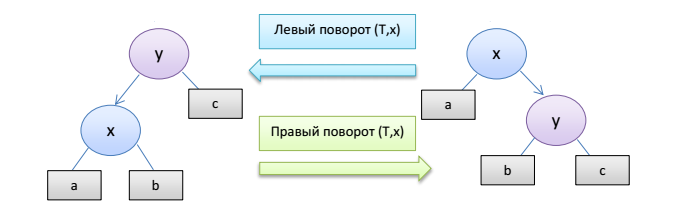
\includegraphics[width=\textwidth]{img/shift.png}
			\caption{Пример левого и правого поворотов.}
		\end{figure}

		\underline{Замечание}

		При выполнении левого поворота в узле X предполагается, что
		его правый ребенок Y не является черным узлом.
	
		При выполнении правого поворота в узле Y предполагается, что
		его левый ребенок X не является черным узлом.

	\section{Алгоритм размещения реплик}	
		Рассматриваемый алгоритм описан в статье <<A Ditributed Algorithm for the Replica Placement Problem>>~\cite{DGR}.
		Алгоритм называется DGR-алгоритм (Distributed Greedy Replication algorithm).

		\subsection{Описание проблемы}
			В больших распеределенных системах возникают ситуации, когда у одного из серверов ($S$) часто запрашивают объект,
			располагающийся не на этом сервере, а на другом удаленном сервере ($R$). В таком случае, при каждом запросе объекта
			распределенная система ищет объект на одном из серверов. Это подразумевает достаточно много сетевых запросов и 
			соответственно увеличивает время выполнения исходного запроса. Если разместить реплику этого объекта на сервере $S$,
			то можно существенно сократить время ожидания объекта на клиенте. DGR-алгоритм позволяет разместить объекты и их
			копии на тех серверах, которые часто запрашивают эти объекты. 

		\subsubsection{Описание алгоритма}
			Определим $m$ --- количество серверов в системе. $n$ --- количество объектов. $s_1, ..., s_m$ --- сервера с емкостями
			$c_1, ..., c_m$. $o_1, ..., o_n$ --- объекты в системе. $t_l$ --- стоимость доступа к объекту, который находится на 
			этом же сервере. $t_r$ --- стоимость доступа к объекту, который находится на другом сервере в группе. $t_s$ --- стоимость 
			доступа к объекту, который находится вне группы. Очевидно, что $t_l \leq t_r \leq t_s$. Каждый сервер $s_i$ знает свой
			коэффициент запросов $r_ij$ для всех $j = 1, ..., n$. Определим матрицу $r$ с элементами $r_ij$, где $i = 1, ..., m$,
			$j = 1, ..., n$ и означает количество запросов объекта $j$ с сервера $i$. Также определим матрицу $X$ с элементами 
			$X_ij$, где $i = 1, ..., m$, $j = 1, ..., n$ и содержит $1$ если объект $j$ хранится на сервере $i$ и $0$  в противном случае.
			Популярность объекта $j$ определяется как общее количество запросов этого объекта со всех серверов $p_j = \sum_{i=1}^{m} r_ij$.
			Количество копий объекта $j$ определяется как $rc_j = \sum_{i=1}^{m} X_ij$.
			Выгода от вставки объекта определяется следующей формулой: 
			 \[ 	
				ig_{ij} =
				\begin{cases} 
			 		p_j (t_s - t_r) + r_{ij} (t_r - t_l) 	& rc_j = 0 \\
			 		r_{ij} (t_r - t_l) 						& X_{ij} = 0, rc_j > 0 \\
			 		0 										    & X_{ij} = 1 
			  	\end{cases}
			 \]
			Стоимость исключения объекта определяется следующей формулой:
			\[ 	
				ec_{ij} =
				\begin{cases} 
					0										& X_{ij} = 0 \\
					r_{ij} (t_r - t_l) 						& X_{ij} = 1, rc_j > 0 \\
					p_j (t_s - t_r) + r_{ij} (t_r - t_l)	& X_{ij} = 1, rc_j = 1 
			 	\end{cases}
			\]


			\begin{algorithm}[tbp]\footnotesize
				\caption{DGR($r, c, t_s , t_r , t_l$)}\label{alg:Example}
				\begin{algorithmic}[1]
					\State \{Server $s_i$\}
					\State \{Initialization\}
					\State \textbf{all-reduce-sum}($r_i, p$)
					\State $X_i \gets 0; e_i \gets c_i$
					\For {$j := 1$ to $n$}
						\State $ig_{ij} \gets p_j (t_s - t_r) + r_{ij} (t_r - t_l); ec_{ij} \gets 0; rc_j \gets 0$
					\EndFor
					\State $ig_{max} \gets max_k (ig_{ik}); j \gets arg(max_k(ig_{ik})$
					\State $send\_msg \gets (ig_{max}, i, j, 0)$
					\State \textbf{all-reduce-max}($send\_msg, recv\_msg$)
					\State $(ig_{max}, i', j, j') \gets recv\_msg$
					\State \{$i'$ is the server that has $ig_{max}$ for object $j$; $j'$ is the object to be evicted from server $i'$ (0 if none)\}
					\While {$ig_{max} > 0$}
						\If {$i' = i$}
							\State \{this server has the maximum insertion gain\}
							\State $X_{ij} \gets 1$
							\State $ec_{ij} \gets ig_{ij}; ig_{ij} \gets 0; e_i \gets e_i - 1; rc_j \gets rc_j + 1$
							\If {$j' \neq 0$}
								\State $X_{ij'} \gets 0$
								\State $ig_{ij'} \gets ec_{ij'}; ec_{ij'} \gets 0$
								\State $e_i \gets e_i + 1; rc_{j'} \gets rc_{j'} - 1$
							\EndIf
						\Else
							\State {\{another server has the maximum insertion gain\}}
							\State $rc_j \gets rc_j + 1$
							\If {$X_{ij} = 0$}
								\State $ig_{ij} \gets r_{ij} (t_r - t_l)$
							\Else
								\State $ec_{ij} \gets r_{ij} (t_r - t_l)$
							\EndIf
							\If {$j' \neq 0$}
								\State $rc_j' \gets rc_{j'} - 1$
								\If {$X_{ij'} = 1$ and $rc_{j'} = 1$}
									\State $ec_{ij'} \gets r_{ij'} (t_r - t_l) + p_{j'} (t_s - t_r)$
								\EndIf
							\EndIf
						\EndIf
						\State \{prepare the next iteration\}
						\State $ig_{max} \gets max_k (ig_{ik}); j \gets arg(max_k(ig_{ik})$
						\State $ec_{min} \gets min_k (ec_{ik} : ec_{ik} > 0)$
						\State $j \gets arg(min_k(ec_{ik} : ec_{ik} > 0)$
						\If {$e_i = 0$ or $c_i - e_i \ge n$}
							\If {$ig_{max} \le ec_{min}$}
								\State $ig_{max} \gets 0; j' \gets 0$
							\EndIf
						\Else 
							\State $j' \gets 0$
						\EndIf
						\State $send\_msg \gets (ig_{max}, i, j, j')$
						\State \textbf{all-reduce-max}($send\_msg, recv\_msg$)
						\State $(ig_{max}, i', j, j') \gets recv\_msg$
					\EndWhile
				 
				\end{algorithmic}
			\end{algorithm}

			\newpage
			Алгоритмы выполняются на всех серверах системы одновременно. Когда они доходят до определенных действий, 
			как например операция $all-reduce-max$, они связываются друг с другом и продолжают после получения ответа 
			от других серверов.

			Изначально каждый алгоритм проходит инициализацию. Начальными значениями заполняются матрица $X$ и вектор $e_i$.
			Вычисляется общая популярность объекта $p$. Помимо этого вычисляются выгода от вставки $ig_{ij}$ и стоимость 
			исключения $ec_{ij}$ для каждого объекта. Далее каждый сервер находит максимальную выгоду от вставки объекта $ig_{max}$ и 
			номер объекта $j$, на котором она достигается. Далее, с помощью операции $all-reduce-max$ сервера находят максимальную 
			выгоду от вставки. После этого запускается цикл который будет продолжать выполняться пока в системе есть объекты, 
			которые выгодно вставить на один из серверов. Если алгоритм запущен на том сервере, на котором необходимо произвести 
			вставку --- $i'$, то создаем реплику объекта $j$. Если при этом с этого же сервера нужно удалить объект $j'$, то 
			удаляем его. Если же алгоритм запущен на другом сервере, то увеличиваем общее количество копий объекта $j$, т.к. он
			будет добавлен на сервер $i'$. Если объект $j$ уже есть на сервере $i$, то изменяем его стоимость исключения $ec_{ij}$,
			а если его нет, то --- выгоду от вставки $ig_{ij}$. Если объект $j'$ нужно удалить с сервера $i$, то уменьшаем количество 
			обращений к этому объекту и если объект расположен на этом сервере и количество копий теперь равно $1$, то просто обновляем
			его стоимость исключения, иначе удаляяем объект. После этого каждый сервер подготавливается к следующей итерации.
			Производится вычисление максимальной выгоды от вставки объекта $ig_{max}$ и номера объекта $j$ на котором это достигается, а также 
			минимальной стоимости исключения $ec_{min}$ и номер объекта $j'$. Если на сервере нет свободного места, или на сервере хранится 
			не меньше чем $n$ объектов и при выполнении этого условия максимальная выгода от вставки $ig_{max}$ меньше чем минимальная стоимость 
			исключения $ec_{min}$, то обнуляем $ig_{max}$ и $j'$. Если даже первое условие не выполняется, то обнуляем только ноиер объекта 
			кандидата на исключение $j'$. Далее сервера снова обмениваются сообщениями, находят максимальную выгоду от вставки и
			переходят к новой итерации.
\newpage

\chapter{Описание распределенной системы}
	Распределенная система, которая была использована в этой работе, состоит из следующих компонент:
	\begin{enumerate}
		\item Сервер
		\item Клиент
		\item Процесс запуска
		\item Процесс барьера
	\end{enumerate}
	Рассмотрим задачи каждой компоненты.

	\section{Сервер}
		Сервер --- это Erlang процесс, который хранит в себе пары ключ-значение, устанавливаемые клиентом, список серверов-соседей, а также
		данные, необходимые для работы алгоритма размещения реплик. 
		
		Сервер S2 является соседом для сервера S1 если между серверами S1 и S2 есть связь.
		
		Из оболочки Erlang серверу можно задавать команды на запуск сервера, его остановку,
		привязку текущего сервера к другому севреру, а также отвязку текущего сервера от другого сервера. Рассмотрим их подробнее.

		\subsection{Запуск сервера}
			\begin{lstlisting}
server:start(name, capacity, barrierPid)
			\end{lstlisting}
			где $name$ - имя сервера, capaity - его емкость, а $barrierPid$ - идентификатор процесса барьера.
			
			Эта команда запускает сервер с заданными параметрами. Для простоты в каждой оболочке запускается только один сервер, так как
			для идентификации сервера в системе используется имя процесса и имя оболочки, в которой этот процесс запущен.

			Результатом команды является идентификатор процесса запущенного сервера.

		\subsection{Остановка сервера}
			\begin{lstlisting}
server:stop()
			\end{lstlisting}
			Эта команда пытется остановить сервер и получает сообщение-результат. Это может быть код ошибки
			\begin{lstlisting}
{error, stopping_this_node_breaks_the_system_into_two_components}
			\end{lstlisting}
			который сообщает о том, что остановка этого сервера разобъет систему на две компоненты. В случае остановки этого сервера
			объекты из одной компоненты будут недоступны клиентам из другой. Другим возможным результатом является сообщение об успешной
			остановке сервера
			\begin{lstlisting}
{ok, stopped}
			\end{lstlisting}

		\subsection{Привязка к соседу}
			\begin{lstlisting}
server:slink(neighbor)
			\end{lstlisting}
			где $neighbor$ - имя Erlang оболочки сервера соседа.

			При выполнении этой команды сервер связывет Erlang оболочки (свою и потенциального соседа), вносит имя Erlang оболочки сервера соседа 
			в список соседей, а после отправляет сообщение о привязке соседу, чтобы он внес текущей сервер в свой список соседей. Результатом команды 
			является сообщение 
			\begin{lstlisting}
{ok, linked}
			\end{lstlisting}
			которое говорит о том, что привязка произошла успешно.

		\subsection{Отвязка от соседа}
			\begin{lstlisting}
server:sunlink(neighbor)
			\end{lstlisting}
			где $neighbor$ - имя Erlang оболочки сервера соседа.

			При выполнении этой команды первым делом проверяется были ли связаны сервера. Если сервера не были связаны, то ответом будет сообщение
			\begin{lstlisting}
{error, servers_are_not_linked}
			\end{lstlisting}
			Если же сервера были связаны, то проверяется, не приведет ли отвязка к разбиению системы на две компоненты. Если приведет, то отвязка не 
			производится и возвращается сообщение
			\begin{lstlisting}
{error, this_link_is_bridge_between_components}
			\end{lstlisting}
			В противном случае сервер удаляетя из списка соседей, а также ему отправляется сообщение об удалении из списка соседей без проверок
			исходного сервера. Результатом в таком случае будет сообщение
			\begin{lstlisting}
{ok, unlinked}
			\end{lstlisting}
			


	\section{Клиент}
		Клиент --- это Erlang процесс, который может привязаться к определенному серверу, установить серверу пару ключ-значение,
		запросить значение по ключу, а также прекратить свою работу. В ходе выполнения любой из вышеперечисленных операций клиент посылает сообщение
		процессу сервера и ожидает ответа. При запуске клиенту необходим сервер, так как любой клиент может обращаться только к одному серверу.
		Установка пары ключ-значение не производит проверок, есть ли данные с таким ключом в системе, а просто перезаписывает значение по заданному 
		ключу на новое. При запросе значения по ключу клиент обращается к единственному известному ему серверу. Тот ищет необходимую пару ключ-значения 
		в данных, которые хранятся у него, и если не находит, обращается ко всем своим соседям, пока не найдет нужный объект. Как только сервер найдет
		необходимую пару он отправит значение, которое и запрашивал клиент. Останавливая свою работу клиент просто останавливает свой процесс не оповещая
		сервер.


	\section{Процесс запуска}
		Процесс запуска --- это Erlang процесс, который запускается первом при старте оболочки Erlang. При запуске он принимает на вход IP-адрес и порт 
		машины, на которую нужно отправить HTTP PUT запрос /register с телом вида shell\_name@ip, где shell\_name - имя оболочки Erlang, а ip - IP адрес
		текущей машины. После этого, процесс ожидает HTTP запросы которые будут управлять настройкой конфигурации системы. Эти запросы могут запускать
		сервер, процесс барьера, связывать и отвязывать сервера друг от друга, а ткаже останавливать их. Это позволяет изменять связи между серверами 
		в процессе работы системы. Помимо этого, благодаря реализации сервера все изменения способные нарушить целостность системы будут отменены.
	

	\section{Процесс барьера}
		Процесс барьера --- это Erlang процесс, который участвует в работе алгоритма размещения реплик. Он необходим для коллективных решений серверов в системе,
		в частности это операция $all-reduce-max$. Каждый из серверов доходя до выполнения этой операции отправляет процессу барьера свои данные, Процесс барьера
		после получения данных от первого сервера в течении определенного времени (50 миллисекунд), а после этого находит присланное сообщение с максимальной 
		выгодой от вставки и отправляет его каждому серверу, который прислал свои данные за этот период. Те сервера, что не успели прислать свои данные процессу 
		барьера перестают участвовать в работе алгоритма размещения реплик и возвращаются к своей обычной работе.Каждый из серверов при старте получает имя оболочки
		Erlang процесса барьера. Было принято решение реализовать принятие решений о максимальном сообщении между серверами с помощью одного отдельного процесса,
		для упрощения реализации алгоритма. Помимо этого процесс барьера позволяет реализовать операцию $all-reduce-max$ быстрее чем при общении между серверами,
		так как время на установку соединения тратится только один раз - в момент запуска сервера, а не при каждом обмене сообщениями.
		

\newpage

\chapter{Детали реализации}
	\section{Клиент}
		Клиент запускается с именем оболочки Erlang на которой располагается сервер, к которому будет обращаться запущенный клиент.
		\begin{lstlisting}
client:cstart(ServerName).			
		\end{lstlisting}
		где $ServerName$ - имя оболочки Erlang сервера. В момент запуска оболочки Erlang клиента и сервера связываются и в текущей оболочке запускается процесс,
		который хранит в своем состоянии $ServerName$. Пользователь выполняет следующие команды
		\begin{lstlisting}
client:set(Key, Vaue).			
client:get(Key).			
client:dgr().			
client:stop().			
		\end{lstlisting}
		которые отправляют процессу клиента следующие сообщения
		\begin{lstlisting}
{self_set, Pid, Key, Value}.			
{self_get, Pid, Key}.			
dgr.			
self_stop.			
		\end{lstlisting}	
		где $Pid$ это идентификатор процесса пользовательского интерфейса клиента, чтобы отослать ему ответ операции. 
		
		Процесс клиента запускакет цикл с единственным параметром --- $ServerName$. 
		\begin{lstlisting}
loop(ServerName) -> 
  receive
    self_stop ->
      handleMessage(self_stop, ServerName);
    Message -> 
      handleMessage(Message, ServerName), 
      loop(ServerName)
  end.
		\end{lstlisting}
		При получении сигнала $self\_stop$ процесс клиента обрабатывает сообщение об остановке и прекращает вызовы функции $loop(ServerName)$. При любом другом сигнале ---
		сообщение обрабатывается и после этого процесс еще раз выполняет $loop(ServerName)$ после чего начинает ожидать новых сообщений от пользователя.

		Функция $handleMessage$ обрабатывает пришедшие процессу клиента сообщения. Она использует сопоставление по шаблону Erlang. В зависимости от аргументов пришедших в функцию
		выбирается соответсвующая реализация. Для примера рассмотрим случаи запроса значения по ключу и остановки клиента. Запросы на установку пары ключ-значение и запуск
		алгоритма размещения реплик аналогичны.
		\begin{lstlisting}
handleMessage({self_get, Pid, Key}, ServerName) ->
  {serverPid, ServerName} ! {c_get, self(), Key},
  receive
    {c_get, {Key, Value, _Number}} ->
      Pid ! {get, {Key, Value}};
      Other -> Pid ! {error, server}
  end;
		\end{lstlisting} 
		Первым аргументом в $handleMessage$ всегда является сообщение в зависимости от которого выбирается вариант его обработки, а вторым аргументом является имя оболочки 
		Erlang сервера. Представленный выше код отправляет сообщение процессу сервера о запросе значения по ключу $Key$, а после ожидает ответа. Если ответом пришел кортеж вида
		${c\_get, {Key, Value, Number}}$, то отправляем пользовательскому процессу кортеж вида ${get, {Key, Value}}$. Если же ответом пришло что-либо другое, то пользовательскому 
		процессу будет отправлено сообщение об ошибке ${error, server}$. 

		\begin{lstlisting}
handleMessage(self_stop, _ServerName) -> {ok, client_stopped};			
		\end{lstlisting}
		При получении запроса на остановку процесс клиента просто возвращает сообщение об успешной остановке.

	\section{Сервер и операции с ним}
		Модуль $server$ предоставляет 4 функции для работы.
		\begin{lstlisting}
server:start(Number, Capacity, BarrierPid).
server:slink(ServerName).
server:sunlink(ServerName).
server:stop().			
		\end{lstlisting}

		\subsection{Основной цикл}
			Логика работы процесса сервера анлогична логике работы процесса клиента: запускается функция цикла $loop$, которая в аргументах хранит состояние, и ожидает сообщений.
			\begin{lstlisting}
loop(State) ->
  receive
    Message -> handleMessage(Message, State)
  end.		
			\end{lstlisting}
			где $State$ - состояние сервера. Оно представляет собой кортеж вида
			\begin{lstlisting}
{LinkedServers, Data, Config}			
			\end{lstlisting}
			где $LinkedServers$ это упорядоченное множество на основе красно-черного дерева, которое хранит имена оболочек Erlanga серверов, с котрыми связан текущий сервер,
			$Data$ это упорядоченное множество на основе красно-черного дерева, которое хранит тройки ключ-значение-номер объекта в сети. $Config$ это кортеж, который содержит 
			информацию необходимую для алгоритма размещения реплик и имеет вид
			\begin{lstlisting}
{I, C, E, Ri, Xi}			
			\end{lstlisting}
			где $I$ - номер сервера в сети, $C$ - емкость сервера, $E$ - количество объектов, которые могут поместиться на этом сервере, $Ri$ - список частоты использования
			использования объектов на этом сервере ($Ri[a] = b$ говорит о том, что объект с номером $a$ был запрошен с этого сервера $b$ раз), $Xi$ - список размещения 
			объектов (0 - если объекта нет на этом сервере, 1 - если есть).

			В отличие от реализации обработки сообщений на клиенте, функция $handleMessage$ в зависимости от вида пришедшего сообщения сама определяет вызвыать ли функцию
			$loop$. В зависимости от вида пришедшего сообщения состояние сервера может измениться, например при добавлении объекта или отвязке сервера.

			Процесс обрабатывает следующие виды сообщений:
			\begin{enumerate}
				\item Конфигурации системы
				\item Клиента 
				\item Внутренних операций
				\item Алгоритма размещения реплик
			\end{enumerate}

		\subsection{Сообщения о конфигурации системы}
			\begin{enumerate}
				\item Об остановке сервера
				\item О привязке
				\item Об отвязке	
			\end{enumerate}
			Сервер обрабатывает 2 вида ообщений об остановке: остановка текущего сервера и остановка соседа. 
			
			\begin{lstlisting}
handleMessage({stop, Pid}, 
              State = {Servers, Data, Config, BarrierPid}) -> 
  case isBridgeNode(node(), to_list(Servers)) of
    true  -> 
	  Pid ! {error, stopping_this_node_breaks_the_system_into_two_components},
      loop(State);
    {false, _UsedServers} ->
	  [H | _T] = to_list(Servers),
      {serverPid, H} ! {add_all, Data},
      notifyStop(to_list(Servers), oset:new(), node()),    
      Pid ! {ok, stopped}
  end;				
			\end{lstlisting}
			При получении сообщения об остановке текущего сервера ($stop$) производится проверка, приведет ли остановка данного сервера к разбиению системы на различные компоненты. 
			Если приведет, отвечает сообщением об ошибке, в противном случае - оповещает всех соседей о своей остановке и отвечает сообщением об остановке, а первому соседу из списка 
			отправляет на хранение все свои данные. В обоих случаях после ответа продолжается работа сервера.

			\begin{lstlisting}
handleMessage({s_stopped, Pid, StoppedName, UsedServers}, 
              State = {Servers, Data, Config, BarrierPid}) ->
  NewServers = del_element(StoppedName, Servers),
  {ok, notifyStop, StoppedName, UpdatedUsedServers} = 
    notifyStop(oset:to_list(NewServers), UsedServers, StoppedName),
  Pid ! {s_stopped, UpdatedUsedServers},
  loop({NewServers, Data, Config, BarrierPid});				
			\end{lstlisting}
			При получении сообщения об остановке соседа ($s\_stopped$), сервер убирает этого соседа из своего списка соседей и продолжает свою работу. В этом случае проверок не производится, 
			так как они уже были произведены останавливаемым сервером. 

			\begin{lstlisting}
handleMessage({link, Pid, ServerName}, 
              State = {Servers, Data, 
                      Config = {I, C, E, Ri, Xi}, 
                      BarrierPid}) ->
  OtherComponentMaxNumber = tryToFixNumbers(ServerName, State),
  NewServers = add_element(ServerName, Servers),
  NewConfig = {I, C, E, 
              Ri ++ fillList(OtherComponentMaxNumber, 0), 
              Xi ++ fillList(OtherComponentMaxNumber, 0)},
  increaseRiXi(OtherComponentMaxNumber,
               to_list(Servers), from_list([node()])),
  {serverPid, ServerName} ! {link, node()},   
  Pid ! {ok, linked}
  loop({NewServers, Data, NewConfig, BarrierPid});				
			\end{lstlisting}
			При получении сообщения о привязке ($link$) если сервера в разных компонентах, то находится максимальный номер объекта в компоненте сети сервера к которому нужно привязать текущий, 
			а после этого увеличиваем все номера в текущей компоненте. Это необходимо для того, чтобы после объединения в сети не было двух объектов с одинаковыми номерами. Помимо этого 
			увеличиваем размеры списков $Xi$ и $Ri$, так как индексы этих списков представляют номера объектов в системе. После этого оба сервера вносят друг друга в свои списки соседей. 
			Если же оба сервера были изначально в одной компоненте, то они просто вносят друг друга в список соседей. Дополнительных проверок на то, являтся ли оба сервера уже связанными 
			не производится, так как если сервера уже связаны, то они точно в одной компоненте, и при попытке внести в список соседей, список останется неизменным, так как представляет собой 
			множество. Далее продолжается работа сервера с обновленным списком соседей.

			\begin{lstlisting}
handleMessage({unlink, Pid, ServerName}, 
              State = {Servers, Data, Config, BarrierPid}) ->
  case is_element(ServerName, Servers) of
    false -> 
      Pid ! {error, servers_are_not_linked},
      loop(State);
    true  ->
      ServerList = to_list(del_element(ServerName, Servers)),
      UsedServers = from_list([node()]),
      case linkIsNotBridge(ServerName, ServerList, UsedServers) of
        {false, _UpdatedUsedServers} -> 
          Pid ! {error, this_link_is_bridge_between_components},
          loop(State);
        true ->
          Pid ! {ok, unlinked},
          {serverPid, ServerName} ! {unlink, node()},
          loop({del_element(ServerName, Servers), 
               Data, Config, BarrierPid})
      end
  end.				
			\end{lstlisting}
			При получении сообщения об отвязке ($unlink$) сервер первым делом проверяет были ли сервера связаны. Если нет, то сервер отвечает сообщением об ошибке и возвращается к 
			основному циклу. Если же сервера были связаны, то производится еще одно проверка --- приведет ли данная отвязка к разбиению системы на две компоненты. Если приведет, то
			сервер отвечает сообщением об ошибке и возвращается к основному циклу. Иначе, серверу-соседу отправляется сообщение, для того, чтобы он удалил текущий сервер из своего списка соседей,
			потом на исходном сервере из списка соседей удаляется сервер-сосед. Далее сервер продолжает работу с обновленным списком соседей.

		\subsection{Сообщения от клиента}
			\begin{enumerate}
				\item О добавлении пары ключ-значение
				\item О запросе значения по ключу
				\item О запуске алгоритма размещенияя реплик	
			\end{enumerate}

			\begin{lstlisting}
handleMessage({c_set, Pid, Key, Value}, 
              State = {Servers, _Data, _Config, BarrierPid}) ->
  Object = findObject(Key, State),
  {NewObject, NewData, NewConfig, _BarrierPid} = 
    tryToAddObject(Object, State, Key, Value),
  Pid ! {c_set, NewObject}, 
  loop({Servers, NewData, NewConfig, BarrierPid});				
			\end{lstlisting}
			При получении сообщения о добавлении пары ключ-значение ($c\_set$) сервер ищет объект с заданным ключом в сети. Если объекта не было в сети, то находится номер, который будет присвоен
			новому объекту. Сам объект добавляется на текущий сервер, увеличиваются вектора $Ri$ и $Xi$, а также каждому серверу сети отправляется уведомление о добавлении нового объекта, чтобы
			они увеличили свои вектора $Ri$ и $Xi$. Текущий сервер проставляет вектору $Xi$ единицу в последнюю ячейку. Если же объект с таким ключом уже есть в сети, то тот сервер, на котором 
			хранится этот объект обновляет значение в этом объекте. В обоих случаях сервера продолжают свою работу с обновленными данными.

			\begin{lstlisting}
handleMessage({c_get, Pid, Key}, 
              State = {Servers, Data, Config, BarrierPid}) ->
  Object = findObject(Key, State),
  case Object of 
    value_not_found ->
      Pid ! {c_get, value_not_found},
      loop(State);
    {_K, _V, N} ->
      { I, C, E, Ri, Xi } = Config,    
      OldRiN = getListItem(N, Ri),
      NewRi = replaceListItem(N, OldRiN + 1, Ri),
      NewConfig = { I, C, E, NewRi, Xi },
      Pid ! {c_get, Object},
      loop({Servers, Data, NewConfig, BarrierPid})
  end;				
			\end{lstlisting}
			При получении сообщения о запросе значения по ключу ($c\_get$) сервер ищет объект сначала локально. Если сервер не находит объект в своем хранилище, то начинается поиск на соседях. 
			Для этого сервер проходит список своих соседей передавая им ключ объекта и множество серверов на которых поиск уже был произведен. Первый из списка соседей ищет объект в своих данных
			и если находит, то возвращает объект на сервер, который инициировал поиск. Если же на нем нет объекта с таким ключом, то он тоже проходит всех своих соседей добавляя себя в множество
			серверов на которых поиск уже был произведен. В таком случае ответом будет либо объект, если он есть на одном из серверов сети, либо сообщение $value\_not\_found$, если такого объекта 
			нет в системе. Также если объект был найден, то исходный сервер увеличивает на единицу соответсвующее значение в векторе количество запросов $Ri$. Далее сервер продолжает свою работу.

			\begin{lstlisting}
handleMessage(d_dgr, 
              State = {Servers, Data, 
                      Config = {I, C, E, Ri, Xi}, 
                      BarrierPid}) ->
  BarrierPid ! start,
  UsedServers = add_element(node(), oset:new()),
  {Popularity, UsedServers} = 
    getPopularity(Ri, to_list(Servers), UsedServers),
  {Objects, NewUsedServers} = 
    getAllObjects(to_list(Servers), Data, UsedServers),
  ObjectsList = to_list(Objects),
  dgrNotify(Popularity, ObjectsList, to_list(Servers), UsedServers),
  loop(dgr(State, Popularity, ObjectsList, initiator));				
			\end{lstlisting}
			При получении сообщения о старте алгоритма размещения реплик ($d\_dgr$) сервер отправлет процесу барьера сообщение о старте текущей сессии. После этого он вычисляет вектор 
			популярности объектов, собирая со всех серверов системы вектора количества запросов $Ri$ и суммируя их. Далее он собирает список всех объектов системы и оповещает все сервера о старте 
			работы алгоритма. После этого каждый сервер запускает алгоритм и продолжает работу с новым состоянием, которое получится после завершения работы алгоритма.		
			
		\subsection{Внутренние сообщения и сообщения алгоритма размещения реплик}
			Внутренние сообщения используются для обеспечения второстепенных операций, например обход системы при вычислении вектора популярности объектов ($d\_popul$) или проверка на то,
			приведет ли удаление связи между двумя серверами к разбиению системы на две компоненты ($is\_bridge$).

			В качестве примера рассмотрим сообщение $add\_all$, которое сохраняет объекты с останавливаемого сервера на его первом соседе.
			\begin{lstlisting}
handleMessage({add_all, NewData}, 
              State = {Servers, Data, Config, BarrierPid}) ->
  UpdatedData = oset:union(Data, NewData),
  loop({Servers, UpdatedData, Config, BarrierPid});		
			\end{lstlisting}

	\section{Алгоритм размещения реплик и синхронизация серверов}
		Функции относящиеся к рассматриваемому алгоритму вынесены в Erlang модуль $dgr$. У этого модуля две основные задачи. Первая это запуск и управление алгоритмом размещения реплик.
		Вторая это управление процессом барьера, так как данный процесс прямо относится к алгоритму.

		\subsection{Процесс барьера}
			Процесс барьера запускается в отдельной Erlang оболочке и ожидает сообщение о начале сессии ($start$), после которого он ожидает сообщения определенное количество времени (в данной 
			работе 50 миллисекунд). При получении сообщения вида ${Pid, Msg}$, где $Pid$ это идентификатор процесса сервера который прислал сообщение, а $Msg$ это само сообщение, процесс барьера 
			вносит их в списки идентификаторов и сообщений, и заново запускает таймер остановки. Если за заданное время процес не получил ни одного сообщения, он перестает реагировать на все 
			сообщения которые придут ему до начала следующей сессии. Далее он ищет сообщение с максимальной выгодой от вставки и отсылает его каждому идентификатору процесса сервера из 
			сохраненных за эту сессию. Те сервера что не успели отправить сообщение до конца сессии выбывают из работы алгоритма.

			\begin{lstlisting}
start_barrier() -> 
  register(barrier, spawn(fun() -> loop() end)).

loop() ->
  receive
    start -> mainLoop([], [])
  end.

mainLoop(Pids, Messages) ->
  receive
    {Pid, Msg} -> mainLoop(Pids ++ [Pid], Messages ++ [Msg])
	after ?BARRIER_TIME -> sendResponses(Pids, Messages)           
  end.	
  
sendResponses(Pids, MessageList = []) -> 
  loop();
sendResponses(Pids, Messages = [H | T]) ->
  MaxMessaage = findMaxMessage(Messages, H),
  send(Pids, MaxMessaage).

send([], MaxMessage) -> 
  loop();
send(Pids = [H | T], MaxMessaage) ->
  H ! {d_barrier, MaxMessaage},
  send(T, MaxMessaage).

findMaxMessage(MessageList = [], Msg) -> 
  Msg;
findMaxMessage(MessageList = [H = {HIgMax, HI, HJ, HJ_} | T], 
               Msg = {IgMax, _I, _J, _J_}) when HIgMax > IgMax -> 
  findMaxMessage(T, H);
findMaxMessage(MessageList = [H = {HIgMax, HI, HJ, HJ_} | T], Msg) -> 
  findMaxMessage(T, Msg).
			\end{lstlisting}

			Каждый из процессов сервера связан с процессом барьера. Это противоречит распределенному характеру системы создавая один узел системы привязанный к каждому серверу. Такое решение 
			было принято по следующим прицинам: простота и скорость работы. Простота означает, что реализация алгоритма принятия решений в распределенной системе не является целью данной работы.
			Скорость работы означает, что при коллективном принятии решений пришлось бы увеличить количество отправляемых сообщений, а при выполнении роли барьера сервером, который запустил 
			алгоритм необходимо было бы связать с ним все сервера и так при каждом запуске алгоритма, что так же повлияло бы на скорость работы. Поэтому создание централизованного узла 
			было выбрано как самый оптимальный способ решения данной проблемы. Если процесс барьера будет недоступен, то алгоритм размещения реплик не изменит состояния серверов системы.

		\subsection{Алгоритм размещения реплик}
			Алгоритм запускается с помощью функции 
			\begin{lstlisting}
dgr(State = {Servers,
            Data, 
            Config = {I, C, E, Ri, Xi}, 
            BarrierPid}, 
    Popularity, Objects, Initiator) ->
  MaxNumber = findMaxNumberLocal(0, Objects),
  NewXi = fillList(MaxNumber, 0),
  NewE = C,
  Ig = initIg(Ri, Popularity),
  Ec = fillList(MaxNumber, 0),
  Rc = fillList(MaxNumber, 0),
  {IgMax, J} = findIgMax(Ig),
  SendMsg = {IgMax, I, J, 0},
  RecvMsg = allReduceMax(BarrierPid, SendMsg),
  {NewData, NewConfig} = whileLoop(RecvMsg, 
    BarrierPid, Objects, oset:new(),
    {I, C, NewE, Ri, NewXi}, 
    {Popularity, MaxNumber, Ig, Ec, Rc}, 
    Servers, Initiator),
  {Servers, NewData, NewConfig, BarrierPid}.
			\end{lstlisting}
			где $State$ --- состояние сервера, $Popularity$ --- это список популярности (количество запросов со всех серверов) объектов, $Objects$ --- список объектов системы, $Initiator$
			--- флаг содержащий атомы $initiator$ и $no\_initiator$. Эта функция проводит инициализацию алгоритма. Находится число объектов в сети $MaxNumber$, вектор размещения объектов на
			текущем сервере $Xi$ заполняется нулями, оставшееся на сервере место $E$ заполняется емкостью $C$, далее по формулам заполняется вектор выгод от вставки объектов $Ig$, а вектор
			стоимости исключения объекта $Ec$ и вектор количества копий $Rc$ заполняются нулями. После этого каждый сервер находит объект с максимальной стоимостью, формирует сообщение $SendMsg$ и отправляет 
			его процессу барьера. Далее он ожидает ответа от процесса барьера с сообщением содержащим максимальную выгоду от вставки во всей системе. Если за определенное время (в данной
			работе 100 миллисекунд) ответа не приходит, то считаем что пришло сообщение с нулевой выгодой от вставки, и в таком случае алгоритм остановится. После этого управление передается 
			циклу $whileLoop$, который производит размещение объектов в системе и по остановке алгоритма возвращает измененное состояние сервера. 
			\begin{lstlisting}
whileLoop(RecvMsg = {IgMax, I_, J, J_}, BarrierPid, 
          Objects, Data, Config = {I, C, E, Ri, Xi},
          Buf = {P, MaxNumber, Ig, Ec, Rc}, Servers,
          Initiator) when IgMax > 0 ->
  {NewData, ResXi, ResIg, ResEc, ResE, ResRc} = igIf(
         RecvMsg, Objects, Servers, Data, Config, 
         {P, MaxNumber, Xi, E, Ig, Ec, Rc}),
  {NewIgMax, NewJ} = findIgMax(Ig),
  {NewEcMin, NewJ_} = findEcMin(Ec),
  {ResIgMax, ResJ_} = terminateIf(E, C, MaxNumber, 
                                  NewIgMax, NewJ_, 
                                  NewEcMin),
  SendMsg = {ResIgMax, I, NewJ, ResJ_},
  initiateBarrier(Initiator, BarrierPid),
  NewRecvMsg = allReduceMax(BarrierPid, SendMsg),
  whileLoop(NewRecvMsg, BarrierPid, Objects, NewData, 
            {I, C, ResE, Ri, ResXi}, 
            {P, MaxNumber, ResIg, ResEc, ResRc}, 
            Servers, Initiator);
  
 whileLoop(RecvMsg, BarrierPid, Objects, Data, Config, 
           Buf, Servers, Initiator) -> 
   {Data, Config}.				
			\end{lstlisting}
			Цикл обрабатывает пришедшее сообщение и если выгода от вставки $IgMax$ больше нуля, значит объекты можно разместить лучше и продолжаем работу, а иначе прекрвщаем работу и возвращаем 
			состояние сервера. Далее каждое условие в теле цикла выносится в отдельную функцию. Каждое из условий может изменить некоторое состояние сервера, например вектор размещения объектов 
			$Xi$ и соответсвенно добавить объект на сервер.

			Функция $igIf$ проверяет, выполняется ли данный алгоритм на том серевре, вставка на который дает максимальную выгоду. Если алгоритм размещения реплик выполняется на этом сервере, то
			выбирается следующая реализация:
			\begin{lstlisting}
igIf(RecvMsg = {IgMax, I_, J, J_}, 
     Objects, Servers, Data,
     Config = {I, C, E, Ri, Xi},
     Buf = {P, MaxNumber, NewXi, E, 
            Ig, Ec, Rc}) when I_ == I ->
  UpdatedXi = replaceListItem(J, 1, NewXi),
  Object = findObjectWithNumber(Objects, J),
  NewData = add_element(Object, Data),    
  NewEc = replaceListItem(J, getListItem(J, Ig), Ec),
  NewIg = replaceListItem(J, 0, Ig),
  NewE = E - 1,
  NewRc = replaceListItem(J, getListItem(J, Rc) + 1, Rc),
  evictedIfIgSelf(NewData, UpdatedXi, NewIg,
                  NewEc, NewE, NewRc, J_);
			\end{lstlisting}
			Так как необходимо сохранить объект с номером $J$ на сервер $I$, то в векторе $Xi$ этого сервера установим значение элемента $J$ в единицу. После этого объект с номером $J$ добавляется 
			в список данных текущего севрера. После этого выгода от вставки объекта с номером $J$ на сервер $I$ записывается в стоимость его исключения, так как он уже хранится на текущем сервере,
			а выгода от вставки этого объекта на этот же сервер становится равна нулю. Количество оставшегося на сервере места $E$ становится меньше на единицу, а в векторе количества копий $Rc$
			увеличиваем значение копий для объекта с номером $J$ на единицу. Далее проверяется условие на исключение объекта с этого севрера функцией $evictedIfIgSelf$.
			\begin{lstlisting}
evictedIfIgSelf(Data, Xi, Ig, Ec, E, Rc, J) when J =/= 0 ->
  NewXi = replaceListItem(J, 0, Xi),
  NewData = removeObjectByNumber(Data, J),
  NewIg = replaceListItem(J, getListItem(J, Ec), Ig),
  NewEc = replaceListItem(J, 0, Ec),
  NewE = E + 1,
  NewRc = replaceListItem(J, getListItem(J, Rc) - 1, Rc),
  {?IF(NewData =:= {error, no_object_with_current_number}, Data, NewData), 
   NewXi, NewIg, NewEc, NewE, NewRc};
	
evictedIfIgSelf(Data, Xi, Ig, Ec, E, Rc, J) -> 
  {Data, Xi, Ig, Ec, E, Rc}.				
			\end{lstlisting}
			Если есть объект, который необходимо исключить с текущего сервера, то в векторе $Xi$ этого сервера установим значение элемента $J$ в ноль и удалим объект с номером $J$ из списка 
			объектов теукущего сервера. После этого в выгоду от вставки объекта с номером $J$ на сервер $I$ записывается стоимость его исключения, так как он уже не хранится на текущем сервере,
			а стоимость исключения этого объекта с этого же сервер становится равна нулю. Количество оставшегося на сервере места $E$ становится больше на единицу, а в векторе количества копий 
			$Rc$ уменьшаем значение копий для объекта с номером $J$ на единицу и возвращаем измененные данные. Если же объекта на удаление нет, то просто оставляем данные сервера без изменений.

			Вернемся к функции $igIf$. Если она вызывается на сервере, на котором вставка не дает макисмальной выгоды, то выбирается следующая реализация:
			\begin{lstlisting}
igIf(RecvMsg = {IgMax, I_, J, J_}, 
     Objects, Servers, Data,
     Config = {I, C, E, Ri, Xi},
     Buf = {P, MaxNumber, NewXi, E, Ig, Ec, Rc}) ->
  NewRc = replaceListItem(J, getListItem(J, Rc) + 1, Rc),
  {NewIg, NewEc} = replicaIf(getListItem(J, NewXi), 
                             getListItem(J, Ri), J, Ig, Ec),
  {ResultRc, ResultEc} = evictedIfIgOther(J_, NewXi, Ri, P, 
                                          NewRc, NewEc),
  {Data, NewXi, NewIg, ResultEc, E, ResultRc}.				
			\end{lstlisting}
			В векторе количества копий $Rc$ увеличиваем значение копий для объекта с номером $J$ на единицу, так как он был сохранен на другом сервере. Далее проверяется наличие объекта с 
			номером $J$ на текущем сервере с помощью функции $replicaIf$, которая заполняет выгоду от вставки объекта и его стоимость исключения новыми данными. 
			\begin{lstlisting}
replicaIf(Xij, Rij, J, Ig, Ec) when Xij == 0 -> 
  NewIg = replaceListItem(J, Rij * (?TR - ?TL), Ig),
  {NewIg, Ec};

replicaIf(_Xij, Rij, J, Ig, Ec) ->
  NewEc = replaceListItem(J, Rij * (?TR - ?TL), Ec),
  {Ig, NewEc}.				
			\end{lstlisting}
			После этого если есть объект, который необходимо исключить с сервера на котором происходят изменения, мы уменьшаем количество копий объекта с номером $J$ в векторе $Rc$ на единицу.
			Если объект сохранен на текущем сервере ($Xij = 1$) и количество его представлений в сети равно единице ($Rcj = 1$), то обновляем значение стоимости исключения объекта с номером $J$,
			а иначе оставляем его без изменений. В обоих случаях возвращаем данные серверу. Если же объекта, который надо исключить не было, то просто возвращаем данные серверу.
			\begin{lstlisting}
evictedIfIgOther(J, Xi, Ri, P, Rc, Ec) when J =/= 0 ->
  NewRc = replaceListItem(J, getListItem(J, Rc) - 1, Rc),
  case getListItem(J, Xi) == 1 andalso getListItem(J, NewRc) == 1 of
    true  -> 
      Rij = getListItem(J, Ri),
      Pj = getListItem(J, P),
      Value = Rij * (?TR -?TL) + Pj * (?TS - ?TR),
      NewEc = replaceListItem(J, Value, Ec),
      {NewRc, NewEc};
    false -> 
      {NewRc, Ec}
  end;

evictedIfIgOther(J, Xi, Ri, P, Rc, Ec) -> 
  {Rc, Ec}.				
			\end{lstlisting}
			Далее происходит подготовка к следующей итерации алгоритма. Находятся максимальная выгода от вставки $IgMax$ с номером объекта на котором она достигается $J$ и минимальная стоимость 
			исключения обекта $EcMin$ с номером объекта на котором она достигается $J\_$. После этого выполняется функция $terminateIf$.
			\begin{lstlisting}
terminateIf(E, C, N, IgMax, J, EcMin) ->
  case E == 0 orelse C - E >= N of
    true  -> 
      case IgMax =< EcMin of
        true  -> 
          {0, 0};
        false -> 
          {IgMax, J}
      end;
    false -> 
      {IgMax, 0}
end.	
			\end{lstlisting}
			Если на сервере не осталось свободного места ($E = 0$) или уже хранятся как минимум все объекты в сети ($C - E >= N$), то если максимальная выгода от вставки не больше минимальной 
			стоимости исключения обнуляем и максимальную выгоду от вставки и номер исключаемого с этого сервера объекта, а если она строго больше то оставляем их без изменений.
			Если же на сервере есть свободное место и на нем расположены еще не все объекты системы, то обнуляем номер исключаемого объекта. 
			
			Далее из полученных данных формируем сообщение. Сервер который инициировал запуск алгоритма уведомляет процесс барьера о начале новой сессии. Каждый сервер отправляет свое
			сообщение процессу барьера  и ожидает от него ответное сообщение с которым запускается нова итерация алгоритма в том случае если выгода от вставки не была равна нулю.


			
\chapter{Результаты тестовых испытаний}
	\section{Описание тестового окружения}
		Все тестовые испытания с оценкой количества итераций алгоритма на одной машине. В глобальной сети была произведена только проверка работоспособности системы. В ходе тестов были 
		произведены проверки на 100, 500 и 1000 объектов и 6 серверов. Сервера соединины друг с другом. 

		Далее предметом рассмотрения будет количество итераций алгоритма, а не временные показатели. Длительность итерации ограничивается процессом барьера. В течении определенного времени
		этот процесс ожидает сообщений от серверов, а после отправляет ответ каждому ссерверу, начиная тем самым новую итерацию. Поэтому время выполнения алгоритма напрямую зависит от 
		количества итераций алгоритма размещения реплик.
		
		\subsection{Конфигурация вычислительной машины}
			Процессор: Intel Core i7-6700HQ CPU @ 2.60GHz x 8 \\
			Операционная система: Ubuntu 16.04.4 LTS 64-bit \\
			Оперативная память: 16 Gb


		\subsection{Конфигураци сети}	
			Различные виды связей между серверами не влияют на работу алгоритма, так как перед стартом основного цикла, сервера собирают все необходимую для работы алгоритма информацию, а после 
			этого независимо друг от друга выполняют итерации алгоритма. Следовательно при изменении конфигурации сети с полносвязной на кольцевую, или же любую другую не изменит количества 
			итераций. Рассмотрим это на примерах полносвязной сети и сети вида звезда.

			\subsubsection{Полносвязная сеть} 
				Сервера $A$, $B$, $C$, $D$, $E$ и $F$ связаны друг с другом. 
				\begin{figure}[H] 
					\centering 
					\scalebox{.5}{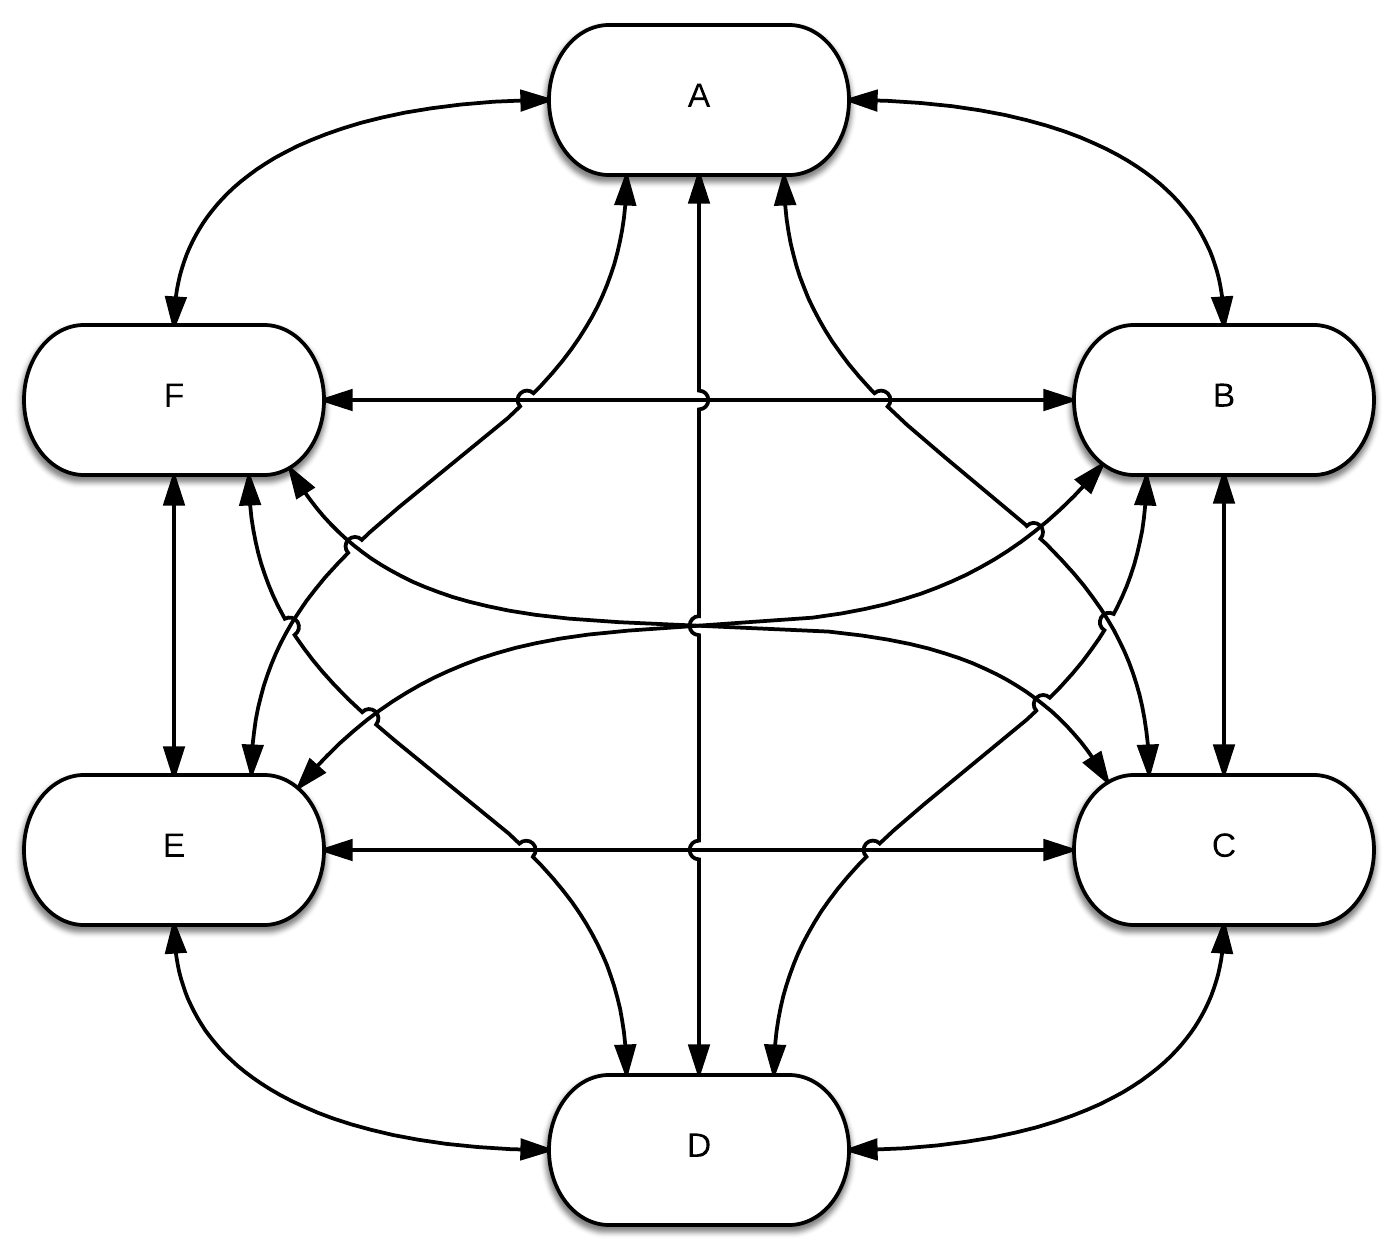
\includegraphics[width=\textwidth]{img/full.png}} 
					\caption{Звезда} 
				\end{figure} 

			\subsubsection{Сеть вида звезда} 
				Сервера $B$, $C$, $D$, $E$ и $F$ связаны только с сервером $A$. 
				\begin{figure}[H] 
					\centering 
					\scalebox{.5}{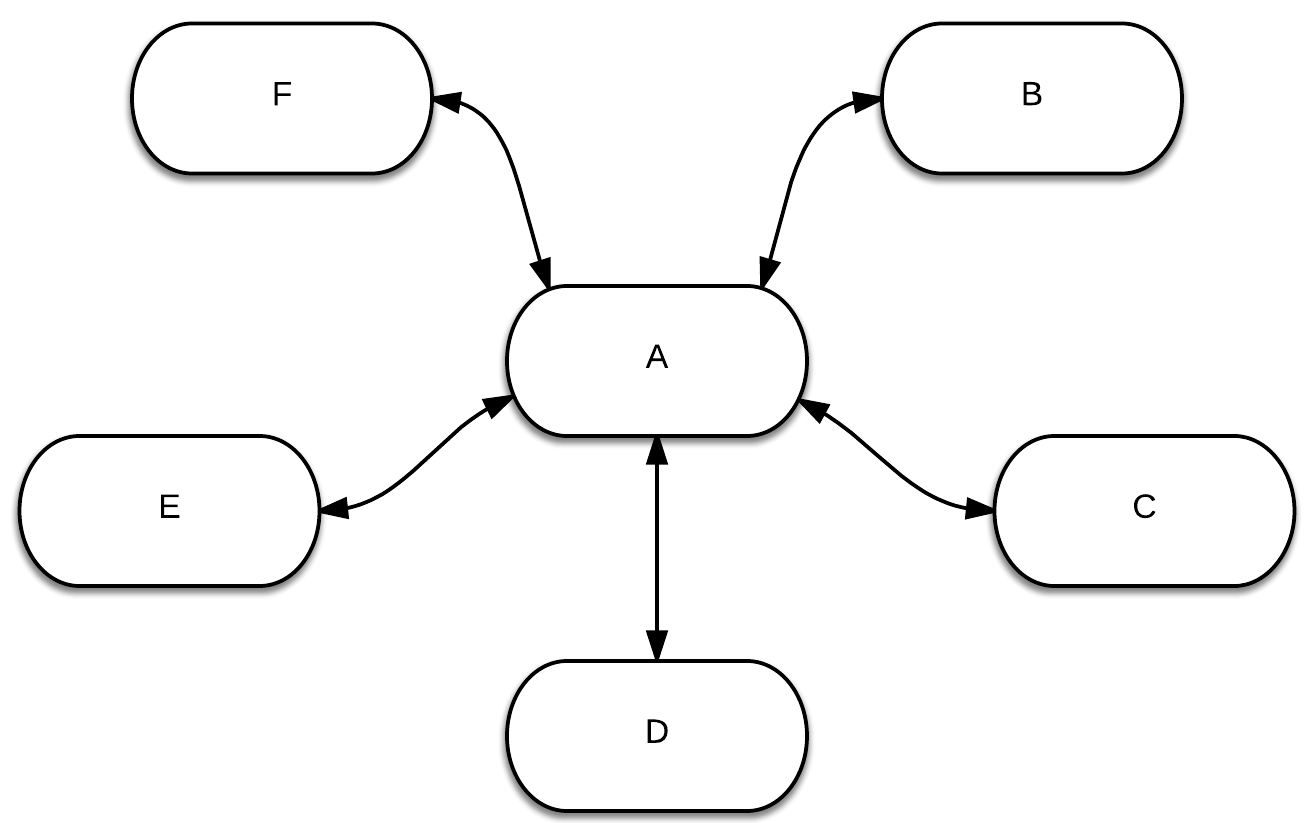
\includegraphics[width=\textwidth]{img/star.png}} 
					\caption{Звезда} 
				\end{figure} 
		
			Было произведено по три испытания для каждого вида сети. В первом испытании в сети содержится 100 объектов и каждый из серверов делает по 500 запросов случайно выбранных объектов.
			Во втором в системе хранится 500 объектов и каждый из серверов делает по 1500 запросов случайно выбранных объектов. В третьем в системе хранится 1000 объектов и каждый из серверов 
			делает по 3000 запросов случайно выбранных объектов. 
			
			Ниже приведена таблица распределения объектов на серверах для каждого из этих трех испытаний:
		
			\begin{table}[H]
				\small
				\centering
				\caption{Таблица размещения объектов}
				\begin{tabular} {|r|c|c|c|c|c|c|}
					\hline
						& A	    & B      & C      & D      & E     & F      \\
					\hline
	100 объектов		& 10    & 20     & 5      & 15     & 40    & 10     \\
	500 объектов		& 70	& 60	 & 70     & 20     & 230   & 50     \\
	1000 объектов		& 1000  & 3000   & 2000   & 1000   & 1500  & 1500   \\
					\hline
				\end{tabular}
			\end{table}
		
			Для данных испытаний рассмотрим количество итераций алгоритма размещения реплик.

			\begin{table}[H]
				\small
				\centering
				\caption{Количество итераций алгоритма размещения реплик}
				\begin{tabular} {|r|c|c|}
					\hline
						& Полносвязная 	& Звезда \\
					\hline
	100 объектов		& 1134			& 1180   \\
	500 объектов		& 3962			& 4195   \\
	1000 объектов		& 7205			& 7572   \\
					\hline
				\end{tabular}
			\end{table}

			Из полученных результатов видно, что смена топологии сети не влияет на работу алгоритма.
			
		\subsection{Количество запросов}
			
		
			Было произведено 6 испытаний. В первом испытании в сети содержится 100 объектов и каждый из серверов делает по 500 запросов случайно выбранных объектов. Во втором --- в сети 
			содержится 100 объектов и каждый из серверов делает по 5000 запросов случайно выбранных объектов. В третьем испытании в сети содержится 500 объектов и каждый из серверов делает 
			по 1500 запросов случайно выбранных объектов. В четвертом --- в сети содержится 500 объектов и каждый из серверов делает по 15000 запросов случайно выбранных объектов. В пятом 
			испытании в сети содержится 1000 объектов и каждый из серверов делает по 5000 запросов случайно выбранных объектов. В шестом --- в сети содержится 1000 объектов и каждый из серверов 
			делает по 10000 запросов случайно выбранных объектов.
			
			Объекты на серверах располагаются аналогично предыдущим испытаниям. Рассмотрим полученное эмпирическим путем количество итераций алгоритма размещения реплик. для каждого испытания.

			\begin{table}[H]
				\small
				\centering
				\caption{Количество итераций алгоритма размещения реплик}
				\begin{tabular} {|r|c|c|}
					\hline
						& Мало запросов & Много запросов \\
					\hline
	100 объектов		& 1180			& 1162 \\
	500 объектов		& 4195			& 4641 \\
	1000 объектов		& 7761			& 8062 \\
					\hline
				\end{tabular}
			\end{table}

			Из полученных результатов видно, что общее количество запросов объекта не влияет на работу алгоритма.

		\subsection{Распределение запросов}
			В предыдущих испытаниях запросы к объектам распределялись равномерно, то есть количество запросов к объектам на одном сервере примерно одинаковое. Сравним количество итераций 
			алгоритма для равномерного и неравномерного распределений. При неравномерном распределении запросов по объектам случайным образом выбирается часть объектов которые у сервера 
			запрашиваются чаще остальных. Причем у каждого сервера эта часть своя.


	
\newpage		
		
\Conc

	В рамках работы изучены принципы функционального программирования, а также реализоваыа распределенная система хранения пар ключ-значения и алгоритм распределения реплик.
	Было произведено сравнение количества итераций алгоритма размещения реплик для различных видов сетей, количества запросов и распределения запросов по объектам сети.
	Помимо этого была проанализирована зависимость количества итераций алгоритма от вышеперечисленных факторов.
\newpage

\printbibliography[%{}
    heading=bibintoc%
]

\end{document}
